\subsubsection{x86: 3 аргумента}

\myparagraph{MSVC}

Компилируем при помощи MSVC 2010 Express, и в итоге получим:

\begin{lstlisting}
$SG3830	DB	'a=%d; b=%d; c=%d', 00H

...

	push	3
	push	2
	push	1
	push	OFFSET $SG3830
	call	_printf
	add	esp, 16					; 00000010H
\end{lstlisting}

Всё почти то же, за исключением того, что теперь видно, что аргументы для \printf заталкиваются в стек в обратном порядке: самый первый аргумент заталкивается последним.

Кстати, вспомним, что переменные типа \Tint в 32-битной системе, как известно, имеет ширину 32 бита, это 4 байта.

Итак, у нас всего 4 аргумента. $4*4 = 16$~--- именно 16 байт занимают в стеке указатель на строку плюс ещё 3 числа типа \Tint.

\myindex{x86!\Instructions!ADD}
\myindex{x86!\Registers!ESP}
\myindex{cdecl}
Когда при помощи инструкции \INS{ADD ESP, X} корректируется \glslink{stack pointer}{указатель стека} \ESP 
после вызова какой-либо функции, зачастую можно сделать вывод о том, сколько аргументов 
у вызываемой функции было, разделив X на 4.

Конечно, это относится только к cdecl-методу передачи аргументов через стек, и только для 32-битной среды.

См. также в соответствующем разделе о способах передачи аргументов через стек ~(\myref{sec:callingconventions}).

Иногда бывает так, что подряд идут несколько вызовов разных функций, но стек корректируется только один раз, после последнего вызова:

\begin{lstlisting}
push a1
push a2
call ...
...
push a1
call ...
...
push a1
push a2
push a3
call ...
add esp, 24
\end{lstlisting}

Вот пример из реальной жизни:

\lstinputlisting[caption=x86]{patterns/03_printf/x86/add_example_RU.lst}

\clearpage
\myparagraph{MSVC и \olly}
\myindex{\olly}

Попробуем этот же пример в \olly.
Это один из наиболее популярных win32-отладчиков пользовательского режима.
Мы можем компилировать наш пример в MSVC 2012 
с опцией \GTT{/MD} что означает линковать с библиотекой \GTT{MSVCR*.DLL},
чтобы импортируемые функции были хорошо видны в отладчике.

Затем загружаем исполняемый файл в \olly.
Самая первая точка останова в \GTT{ntdll.dll}, нажмите F9 (запустить).
Вторая точка останова в \ac{CRT}-коде.
Теперь мы должны найти функцию \main.

Найдите этот код, прокрутив окно кода до самого верха (MSVC располагает функцию \main в самом начале секции кода): 

\begin{figure}[H]
\centering
\myincludegraphics{patterns/03_printf/x86/olly3_1.png}
\caption{\olly: самое начало функции \main}
\label{fig:printf3_olly_1}
\end{figure}

Кликните на инструкции \INS{PUSH EBP}, нажмите F2 (установка точки останова) и нажмите F9 (запустить).
Нам нужно произвести все эти манипуляции, чтобы пропустить \ac{CRT}-код, потому что нам он пока
не интересен.

\clearpage
Нажмите F8 (\stepover) 6 раз, т.е. пропустить 6 инструкций:

\begin{figure}[H]
\centering
\myincludegraphics{patterns/03_printf/x86/olly3_2.png}
\caption{\olly: перед исполнением \printf}
\label{fig:printf3_olly_2}
\end{figure}

Теперь \ac{PC} указывает на инструкцию \INS{CALL printf}.
\olly, как и другие отладчики, подсвечивает регистры со значениями, которые изменились.
Поэтому каждый раз когда мы нажимаем F8, \EIP изменяется и его значение подсвечивается красным.
\ESP также меняется, потому что значения заталкиваются в стек.\\
\\
Где находятся эти значения в стеке?
Посмотрите на правое нижнее окно в отладчике:

\begin{figure}[H]
\centering
\ifdefined\ebook
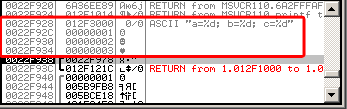
\includegraphics[width=\textwidth]{patterns/03_printf/x86/olly3_stack.png}
\else
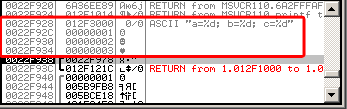
\includegraphics[width=0.5\textwidth]{patterns/03_printf/x86/olly3_stack.png}
\fi

\caption{\olly: стек с сохраненными значениями (красная рамка добавлена в графическом редакторе)}
\end{figure}

Здесь видно 3 столбца: адрес в стеке, значение в стеке и ещё дополнительный комментарий
от \olly. 
\olly понимает \printf{}-строки, так что он показывает здесь и строку и 3 значения \IT{привязанных} к ней.

Можно кликнуть правой кнопкой мыши на строке формата, кликнуть на \q{Follow in dump}
и строка формата появится в окне слева внизу, где всегда виден какой-либо участок памяти.
Эти значения в памяти можно редактировать.
Можно изменить саму строку формата, и тогда результат работы нашего примера будет другой.
В данном случае пользы от этого немного, но для упражнения это полезно,
чтобы начать чувствовать как тут всё работает.

\clearpage
Нажмите F8 (\stepover).

В консоли мы видим вывод:

\lstinputlisting{patterns/03_printf/x86/console.txt}

Посмотрим как изменились регистры и состояние стека: 

\begin{figure}[H]
\centering
\myincludegraphics{patterns/03_printf/x86/olly3_3.png}
\caption{\olly после исполнения \printf}
\label{fig:printf3_olly_3}
\end{figure}

Регистр \EAX теперь содержит \GTT{0xD} (13).
Всё верно: \printf возвращает количество выведенных символов.
Значение \EIP изменилось. Действительно, теперь здесь адрес инструкции после \INS{CALL printf}.
Значения регистров \ECX и \EDX также изменились.
Очевидно, внутренности функции \printf используют их для каких-то своих нужд.

Очень важно то, что значение \ESP не изменилось. И аргументы-значения в стеке также!
Мы ясно видим здесь и строку формата и соответствующие ей 3 значения, они всё ещё здесь.
Действительно, по соглашению вызовов \IT{cdecl}, вызываемая функция не возвращает \ESP назад.
Это должна делать вызывающая функция (\gls{caller}).

\clearpage
Нажмите F8 снова, чтобы исполнилась инструкция \INS{ADD ESP, 10}:

\begin{figure}[H]
\centering
\myincludegraphics{patterns/03_printf/x86/olly3_4.png}
\caption{\olly: после исполнения инструкции \INS{ADD ESP, 10}}
\label{fig:printf3_olly_4}
\end{figure}

\ESP изменился, но значения всё ещё в стеке!
Конечно, никому не нужно заполнять эти значения нулями или что-то в этом роде.
Всё что выше указателя стека (\ac{SP}) 
это \IT{шум} или \IT{\garbage{}} и не имеет особой ценности.
Было бы очень затратно по времени очищать ненужные элементы стека, к тому же, никому это и не нужно.

\myparagraph{GCC}

Скомпилируем то же самое в Linux при помощи GCC 4.4.1 и посмотрим на результат в \IDA:

\begin{lstlisting}
main            proc near

var_10          = dword ptr -10h
var_C           = dword ptr -0Ch
var_8           = dword ptr -8
var_4           = dword ptr -4

                push    ebp
                mov     ebp, esp
                and     esp, 0FFFFFFF0h
                sub     esp, 10h
                mov     eax, offset aADBDCD ; "a=%d; b=%d; c=%d"
                mov     [esp+10h+var_4], 3
                mov     [esp+10h+var_8], 2
                mov     [esp+10h+var_C], 1
                mov     [esp+10h+var_10], eax
                call    _printf
                mov     eax, 0
                leave
                retn
main            endp
\end{lstlisting}

Можно сказать что этот короткий код, созданный GCC, отличается от кода MSVC только способом помещения 
значений в стек.
Здесь GCC снова работает со стеком напрямую без \PUSH/\POP.

\myparagraph{GCC и GDB}
\myindex{GDB}

Попробуем также этот пример и в \ac{GDB} в Linux.

\GTT{-g} означает генерировать отладочную информацию в выходном исполняемом файле.

\begin{lstlisting}
$ gcc 1.c -g -o 1
\end{lstlisting}

\begin{lstlisting}
$ gdb 1
GNU gdb (GDB) 7.6.1-ubuntu
Copyright (C) 2013 Free Software Foundation, Inc.
License GPLv3+: GNU GPL version 3 or later <http://gnu.org/licenses/gpl.html>
This is free software: you are free to change and redistribute it.
There is NO WARRANTY, to the extent permitted by law.  Type "show copying"
and "show warranty" for details.
This GDB was configured as "i686-linux-gnu".
For bug reporting instructions, please see:
<http://www.gnu.org/software/gdb/bugs/>...
Reading symbols from /home/dennis/polygon/1...done.
\end{lstlisting}

\begin{lstlisting}[caption=установим точку останова на \printf]
(gdb) b printf
Breakpoint 1 at 0x80482f0
\end{lstlisting}

Запукаем.
У нас нет исходного кода функции, поэтому \ac{GDB} не может его показать.

\begin{lstlisting}
(gdb) run
Starting program: /home/dennis/polygon/1 

Breakpoint 1, __printf (format=0x80484f0 "a=%d; b=%d; c=%d") at printf.c:29
29	printf.c: No such file or directory.
\end{lstlisting}

Выдать 10 элементов стека. Левый столбец~--- это адрес в стеке.

\begin{lstlisting}
(gdb) x/10w $esp
0xbffff11c:	0x0804844a	0x080484f0	0x00000001	0x00000002
0xbffff12c:	0x00000003	0x08048460	0x00000000	0x00000000
0xbffff13c:	0xb7e29905	0x00000001
\end{lstlisting}

Самый первый элемент это \ac{RA} (\GTT{0x0804844a}).
Мы можем удостовериться в этом, дизассемблируя память по этому адресу:

\begin{lstlisting}[label=NOP_as_XCHG_example]
(gdb) x/5i 0x0804844a
   0x804844a <main+45>:	mov    $0x0,%eax
   0x804844f <main+50>:	leave  
   0x8048450 <main+51>:	ret    
   0x8048451:	xchg   %ax,%ax
   0x8048453:	xchg   %ax,%ax
\end{lstlisting}

Две инструкции \INS{XCHG} это холостые инструкции, аналогичные \ac{NOP}.

Второй элемент (\GTT{0x080484f0}) это адрес строки формата:

\begin{lstlisting}
(gdb) x/s 0x080484f0
0x80484f0:	"a=%d; b=%d; c=%d"
\end{lstlisting}

Остальные 3 элемента (1, 2, 3) это аргументы функции \printf.
Остальные элементы это может быть и мусор в стеке, но могут быть и значения
от других функций, их локальные переменные, \etc{}.
Пока что мы можем игнорировать их.

Исполняем \q{finish}. 
Это значит исполнять все инструкции до самого конца функции. 
В данном случае это означает исполнять до завершения \printf.

\begin{lstlisting}
(gdb) finish
Run till exit from #0  __printf (format=0x80484f0 "a=%d; b=%d; c=%d") at printf.c:29
main () at 1.c:6
6		return 0;
Value returned is $2 = 13
\end{lstlisting}

\ac{GDB} показывает, что вернула \printf в \EAX (13).
Это, так же как и в примере с \olly, количество напечатанных символов.

А ещё мы видим \q{return 0;} и что это выражение находится в файле \GTT{1.c} в строке 6.
Действительно, файл \GTT{1.c} лежит в текущем директории и \ac{GDB} находит там эту строку.
Как \ac{GDB} знает, какая строка Си-кода сейчас исполняется?
Компилятор, генерируя отладочную информацию, также сохраняет информацию о соответствии строк в исходном коде и адресов инструкций.
GDB это всё-таки отладчик уровня исходных текстов.

Посмотрим регистры.
13 в \EAX:

\begin{lstlisting}
(gdb) info registers
eax            0xd	13
ecx            0x0	0
edx            0x0	0
ebx            0xb7fc0000	-1208221696
esp            0xbffff120	0xbffff120
ebp            0xbffff138	0xbffff138
esi            0x0	0
edi            0x0	0
eip            0x804844a	0x804844a <main+45>
...
\end{lstlisting}

Попробуем дизассемблировать текущие инструкции.
Стрелка указывает на инструкцию, которая будет исполнена следующей.

\begin{lstlisting}
(gdb) disas
Dump of assembler code for function main:
   0x0804841d <+0>:	push   %ebp
   0x0804841e <+1>:	mov    %esp,%ebp
   0x08048420 <+3>:	and    $0xfffffff0,%esp
   0x08048423 <+6>:	sub    $0x10,%esp
   0x08048426 <+9>:	movl   $0x3,0xc(%esp)
   0x0804842e <+17>:	movl   $0x2,0x8(%esp)
   0x08048436 <+25>:	movl   $0x1,0x4(%esp)
   0x0804843e <+33>:	movl   $0x80484f0,(%esp)
   0x08048445 <+40>:	call   0x80482f0 <printf@plt>
=> 0x0804844a <+45>:	mov    $0x0,%eax
   0x0804844f <+50>:	leave  
   0x08048450 <+51>:	ret    
End of assembler dump.
\end{lstlisting}

По умолчанию \ac{GDB} показывает дизассемблированный листинг в формате AT\&T.
Но можно также переключиться в формат Intel:

\begin{lstlisting}
(gdb) set disassembly-flavor intel
(gdb) disas
Dump of assembler code for function main:
   0x0804841d <+0>:	push   ebp
   0x0804841e <+1>:	mov    ebp,esp
   0x08048420 <+3>:	and    esp,0xfffffff0
   0x08048423 <+6>:	sub    esp,0x10
   0x08048426 <+9>:	mov    DWORD PTR [esp+0xc],0x3
   0x0804842e <+17>:	mov    DWORD PTR [esp+0x8],0x2
   0x08048436 <+25>:	mov    DWORD PTR [esp+0x4],0x1
   0x0804843e <+33>:	mov    DWORD PTR [esp],0x80484f0
   0x08048445 <+40>:	call   0x80482f0 <printf@plt>
=> 0x0804844a <+45>:	mov    eax,0x0
   0x0804844f <+50>:	leave  
   0x08048450 <+51>:	ret    
End of assembler dump.
\end{lstlisting}

Исполняем следующую инструкцию.
\ac{GDB} покажет закрывающуюся скобку, означая, что это конец блока в функции.

\begin{lstlisting}
(gdb) step
7	};
\end{lstlisting}

Посмотрим регистры после исполнения инструкции \INS{MOV EAX, 0}.
\EAX здесь уже действительно ноль.

\begin{lstlisting}
(gdb) info registers
eax            0x0	0
ecx            0x0	0
edx            0x0	0
ebx            0xb7fc0000	-1208221696
esp            0xbffff120	0xbffff120
ebp            0xbffff138	0xbffff138
esi            0x0	0
edi            0x0	0
eip            0x804844f	0x804844f <main+50>
...
\end{lstlisting}
